%-------------------------------------------------------
\section{Available Data}
%-------------------------------------------------------
\begin{frame}{Raw Data}{What is the nature of the starting material?}
%-------------------------------------------------------

\begin{itemize}

    \item<1->\textbf{Data about \alert{students}}: academic career results of each student during a certain time span \\
        \noindent\begin{centering}
            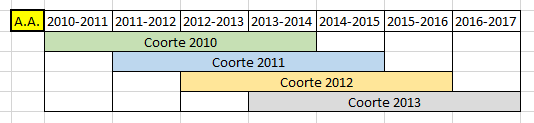
\includegraphics[scale=0.50]{../raw/stud_comp.png}
        \end{centering}

    \item<2->\textbf{Data about \alert{courses}}: teachings evaluations questionary compiled by the students, in an \emph{aggregate} form for each \texttt{<Academical Year, Teaching Course>}.

\end{itemize}

\end{frame}

%-------------------------------------------------------
\section{Data Understanding}
%-------------------------------------------------------
\subsection{Students Data}
%-------------------------------------------------------
\begin{frame}{Data Understanding}{Visualization techniques on students data}

    \vspace{0.2cm}
    \begin{centering}
        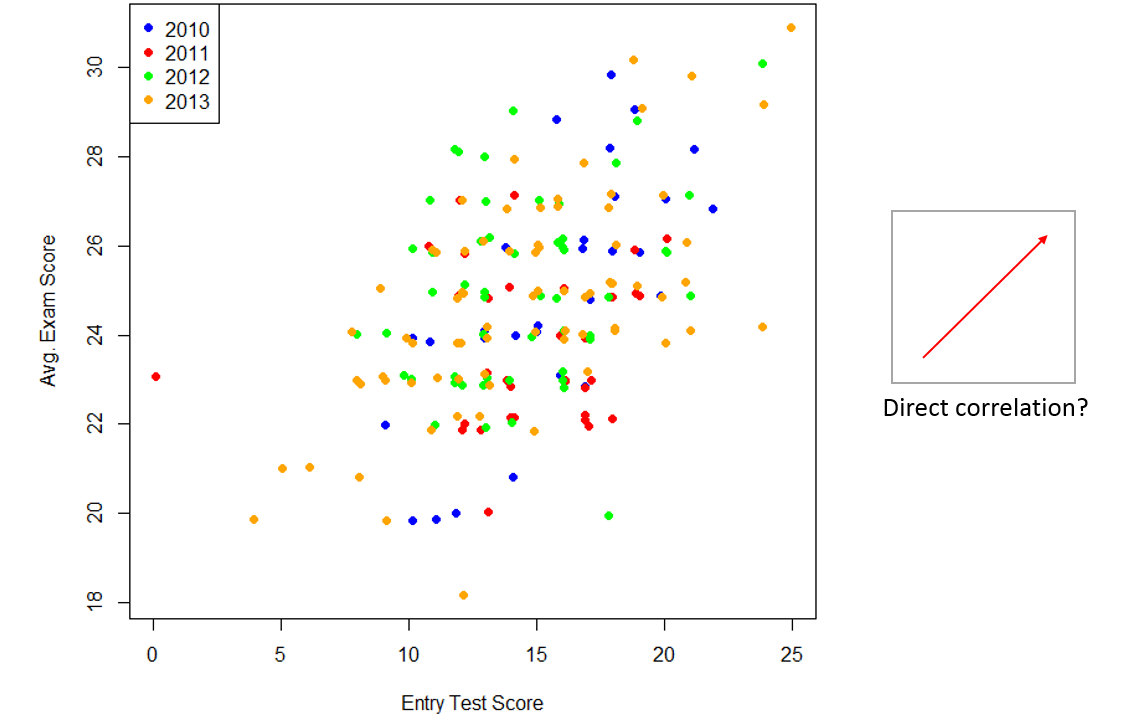
\includegraphics[scale=0.28]{img2_noback.png}
    \end{centering}

\end{frame}

\begin{frame}{Data Understanding}{Visualization techniques on students data}

    \vspace{0.5cm}
    \noindent\begin{centering}
        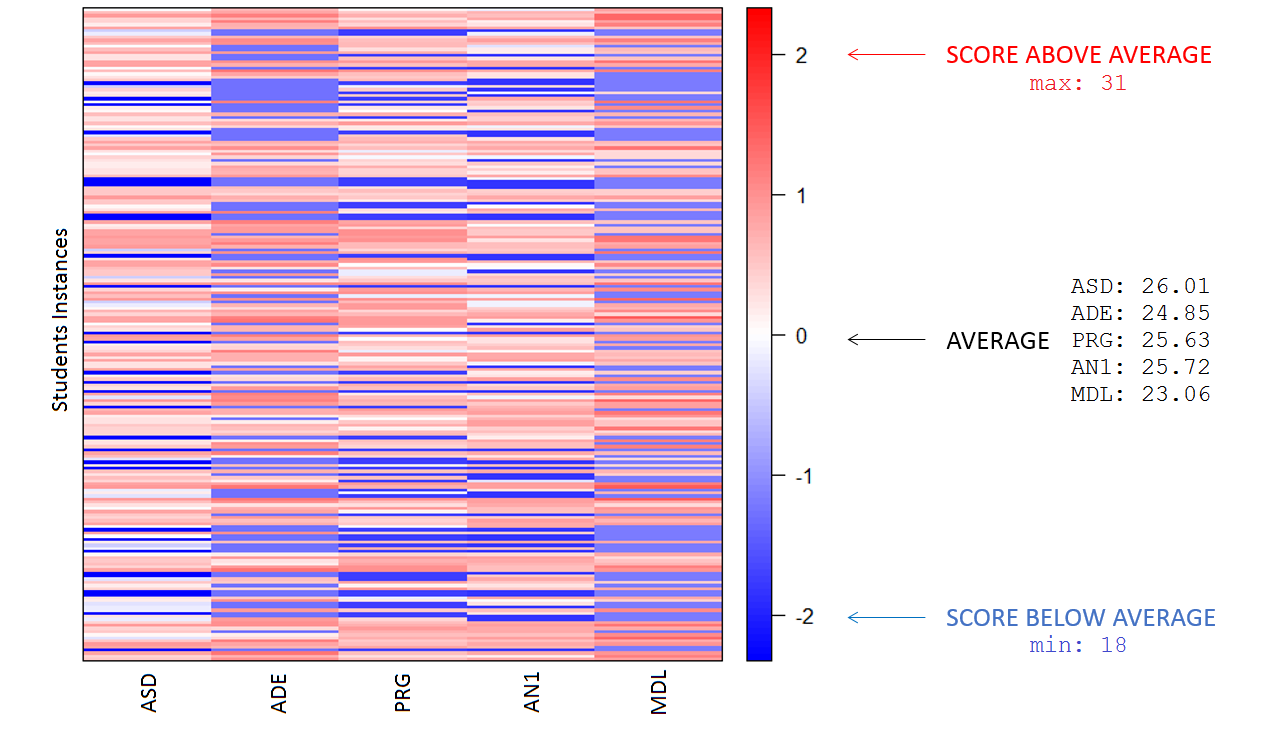
\includegraphics[scale=0.25]{img3.png}
    \end{centering}

\end{frame}

\begin{frame}{Data Understanding}{Visualization techniques on students data}

    \vspace{0.5cm}
    \hspace*{-0.8cm}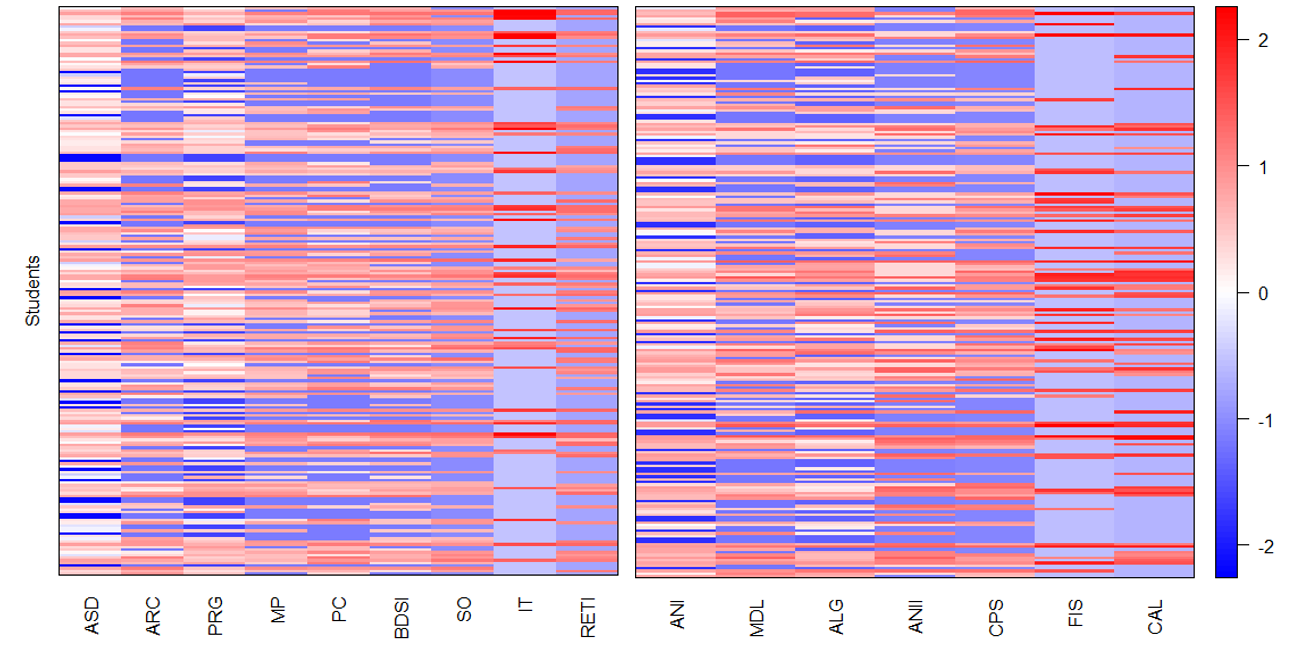
\includegraphics[scale=0.275]{img4.png}

\end{frame}